\section{Introduction}
\label{sec:intro}

\begin{figure}[t]
    \centering
    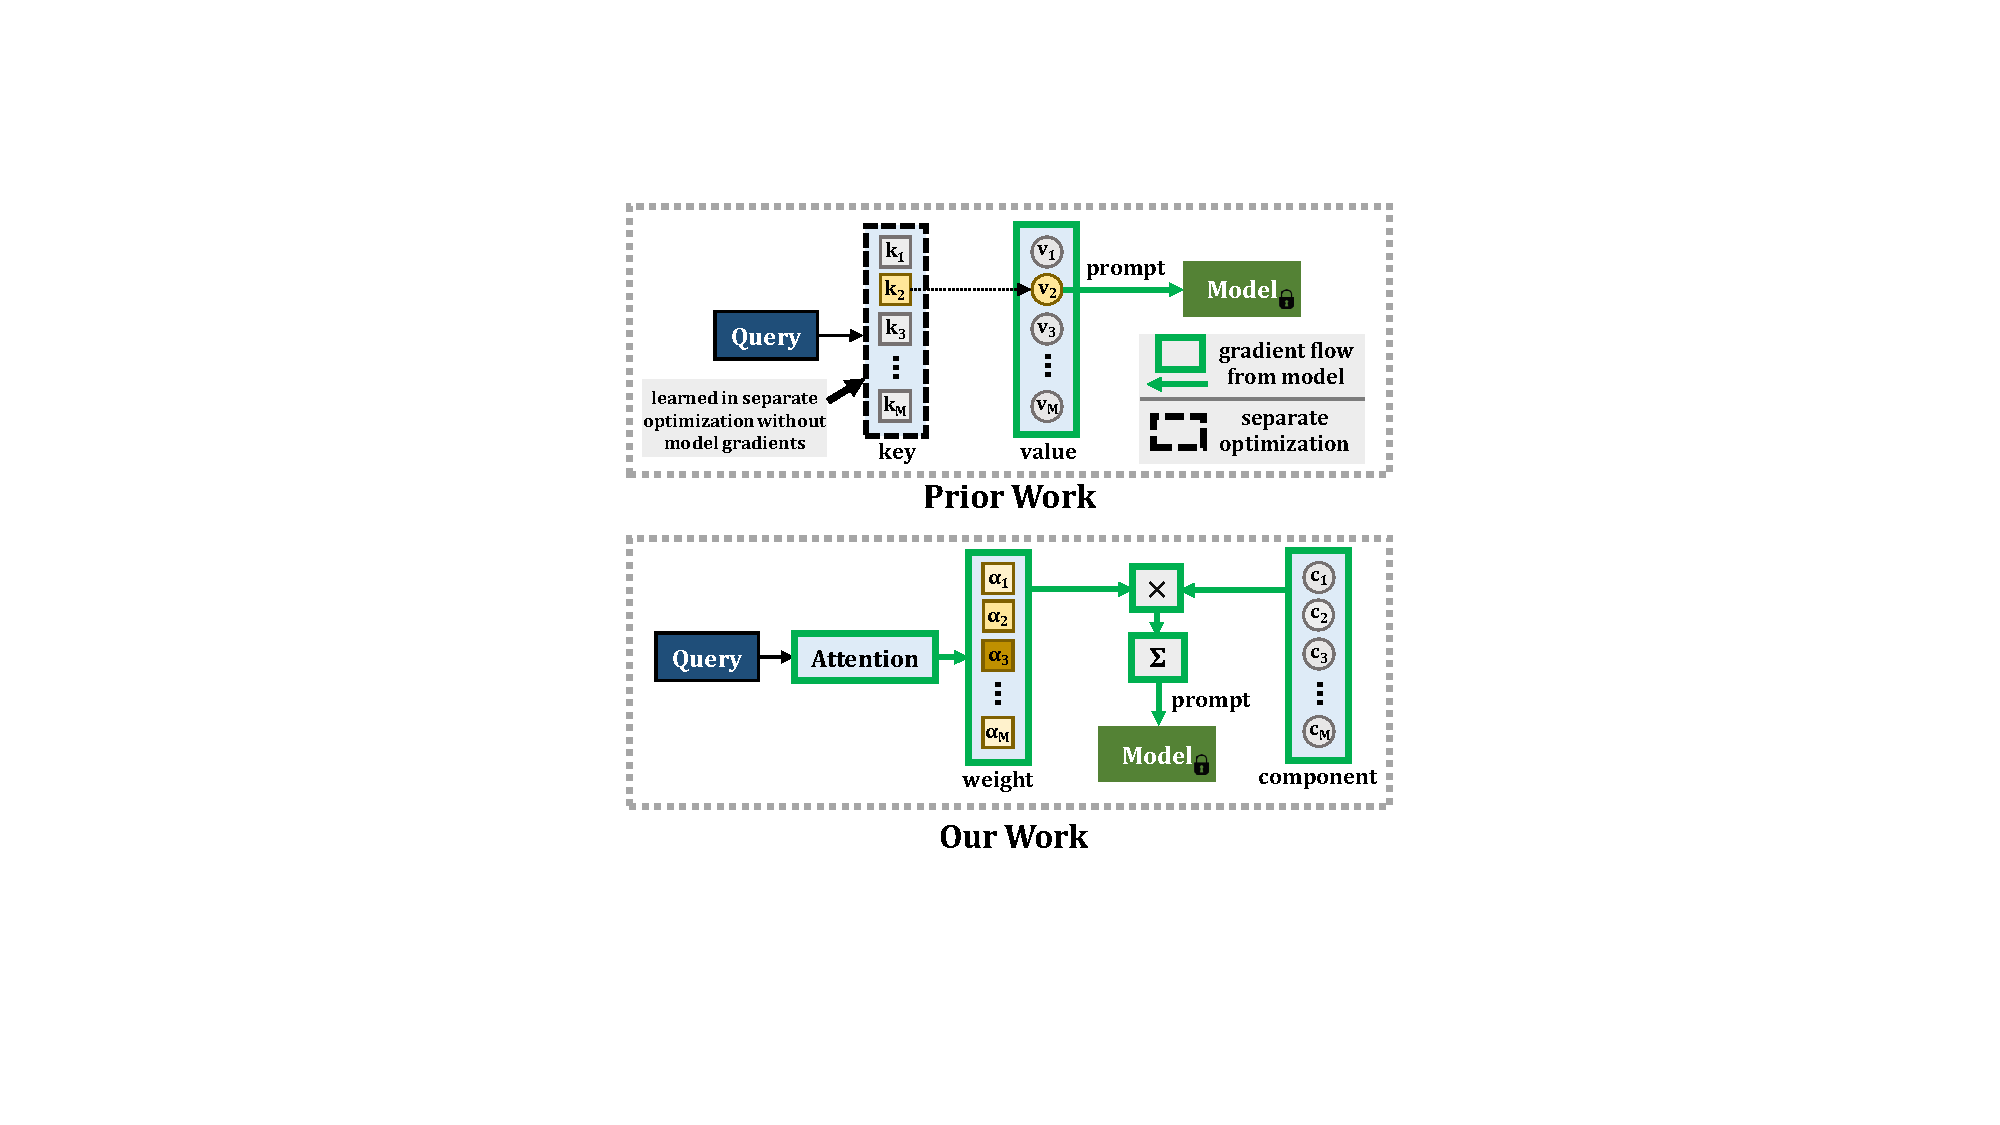
\includegraphics[width=0.46\textwidth]{figures/source/key_idea.pdf}
    \caption{\textbf{Prior work}~\cite{wang2022dualprompt} learns a pool of key-value pairs to select learnable prompts which are inserted into several layers of a pre-trained ViT (the prompting parameters are unique to each layer). \textbf{Our work} introduces a \textbf{decomposed prompt} which consists of learnable prompt \emph{components} that assemble to produce \emph{attention-conditioned} prompts. Unlike prior work, ours is \textbf{optimized in an end-to-end fashion} (denoted with thick, green lines).
    }
    \label{fig:key-idea}
    \vspace{-3mm}
\end{figure}






\vspace{-2mm}
For a computer vision model to succeed in the real world, it must overcome brittle assumptions that the concepts it will encounter after deployment will match those learned \emph{a-priori} during training. The real world is indeed \emph{dynamic} and contains continuously emerging objects and categories. Once deployed,  models will encounter a range of differences from their training sets, requiring us to continuously update them to avoid stale and decaying performance.


One way to update a model is to collect additional training data, combine this new training data with the old training data, and then retrain the model from scratch. While this will guarantee high performance, it is not practical for large-scale applications which may require lengthy training times and aggressive replacement timelines, such as models for self-driving cars or social media platforms. This could incur \emph{high financial~\cite{justus2018predicting} and environmental~\cite{lacoste2019quantifying} costs} if the replacement is frequent. We could instead update the model by only training on the new training data, but this leads to a phenomenon known as \emph{catastrophic forgetting}~\cite{nguyen2019toward} where the model overwrites existing knowledge when learning the new data, a problem known as %
\emph{continual learning}.

The most effective approaches proposed by the continual learning community involve saving~\cite{Rebuffi:2016} or generating~\cite{Shin:2017} a subset of past training data and mixing it with future task data, a strategy referred to as \textbf{rehearsal}. Yet many important applications are unable to store this data because they work with \emph{private user data that cannot be stored} long term.%

In this paper, we instead consider the highly-impactful and well-established setting of \emph{rehearsal-free} continual learning\cite{wang2022learning,wang2022dualprompt,smith2021abd,smith2022closer,li2016learning}\footnote{We focus on continual learning over a single, expanding classification head called \textit{class-incremental continual learning}. This is different from the multi-task continual learning setting, known as \textit{task-incremental} continual learning, where we learn separate classification heads for each task and the task label is provided during inference.\cite{hsu2018re,van2019three}}, limiting our scope to strategies for continual learning which do not store training data. While rehearsal-free approaches have classically under-performed rehearsal-based approaches in this challenging setting by wide-margins~\cite{smith2022closer}, recent \emph{prompt-based approaches}~\cite{wang2022learning,wang2022dualprompt}, leveraging pre-trained Vision transformers (ViT), have had tremendous success and can even outperform state-of-the-art (SOTA) rehearsal-based methods. These prompting approaches boast a strong protection against catastrophic forgetting by learning a small pool of insert-able model embeddings (prompts) rather than modifying vision encoder parameters directly. One drawback of these approaches, however, is that they cannot be optimized in an \emph{end-to-end} fashion as they use a key and query to select a prompt \emph{index} from the pool of prompts, and thus rely on a second, localized optimization to learn the keys because the model gradient cannot backpropagate through the key/query index selection.
Furthermore, these methods reduce forgetting by \emph{sacrificing new task accuracy} (i.e., they lack sufficient \emph{plasticity}). We show that expanding the prompt size does not increase the plasticity, motivating us to grow learning capacity from a new perspective.


We replace the prompt pool with a \emph{decomposed prompt} that consists of a weighted sum of learnable prompt components (Figure~\ref{fig:key-idea}). This decomposition enables higher prompting capacity by expanding in a new dimension (the number of components). Furthermore, this inherently encourages knowledge re-use, as future task prompts will include contributions from prior task components. We also introduce a novel attention-based component-weighting scheme, which allows for our entire method to be \emph{optimized in an end-to-end fashion} unlike the existing works, increasing our plasticity to better learn future tasks. 
We boast significant performance gains on existing rehearsal-free continual learning benchmarks w.r.t. SOTA prompting baselines in addition to a challenging \emph{dual-shift} benchmark containing both incremental concept shifts \emph{and} covariate domain shifts, highlighting our method's impact and generality. Our method improves results even under equivalent parameter counts, but importantly can scale performance by increasing capacity, unlike prior methods which quickly plateau. 
\emph{In summary, we make the following contributions:}
\begin{enumerate}
    \item We introduce a \emph{decomposed} attention-based prompting for rehearsal-free continual learning, characterized by an \emph{expanded learning capacity} compared to existing continual prompting approaches. Importantly, our approach can be optimized in an end-to-end fashion, unlike the prior SOTA.
    \item We establish a new SOTA for rehearsal-free continual learning on the well-established ImageNet-R~\cite{hendrycks2021many,wang2022dualprompt} and CIFAR-100~\cite{krizhevsky2009learning} benchmarks, beating the previous SOTA method DualPrompt~\cite{wang2022dualprompt} by as much as 4.5\%.
    \item We evaluate on a challenging benchmark with dual distribution shifts (semantic \emph{and} covariate) using the ImageNet-R dataset, and again outperform the state of art, highlighting the real-world impact and generality of our approach.
\end{enumerate}
